\newcommand{\PraxisTeam}{7391857}
\newcommand{\PraxisTitle}{Paying for the Bottleneck: A Compatible-Flow Design for Toll-Plaza Merging}
% BEGIN PRAXIS MCM STYLE v1
% Praxis MCM house style v1. Layout source; assemble with scripts.paper_template.
\documentclass[12pt,letterpaper]{article}
\usepackage[left=1in,right=1in,top=0.95in,bottom=0.8in,headheight=15pt]{geometry}
\usepackage{amsmath,amssymb,amsthm}
\usepackage{newtxtext,newtxmath}
\usepackage{booktabs,array,graphicx,xcolor,caption,float,etoolbox,fvextra,fancyhdr,lastpage,titlesec,titletoc,needspace}
\usepackage[hidelinks,pdfauthor={},pdftitle={\PraxisTitle}]{hyperref}
\urlstyle{same}\Urlmuskip=0mu plus 1mu
\usepackage{pgfplots}
\pgfplotsset{compat=1.17}
\usepgfplotslibrary{fillbetween,groupplots}
\usetikzlibrary{arrows.meta,positioning,calc}
\definecolor{main}{HTML}{0072B2}
\definecolor{accent}{HTML}{D55E00}
\definecolor{muted}{HTML}{7A7F85}
\definecolor{light}{HTML}{B8BDC2}
\definecolor{oigreen}{HTML}{009E73}
\definecolor{oiorange}{HTML}{E69F00}
\definecolor{oisky}{HTML}{56B4E9}
\definecolor{oiyellow}{HTML}{F0E442}
\definecolor{teal}{HTML}{17766E}
\definecolor{clay}{HTML}{9E6440}
\definecolor{slate}{HTML}{5D696E}
\definecolor{sand}{HTML}{AAA69B}
\linespread{1.12}
\setlength{\parindent}{1.5em}\setlength{\parskip}{3pt}
\titleformat{\section}{\Large\bfseries}{\thesection}{0.6em}{}
\titleformat{\subsection}{\large\bfseries}{\thesubsection}{0.6em}{}
\titlespacing*{\section}{0pt}{16pt plus 3pt}{8pt}
\titlespacing*{\subsection}{0pt}{12pt plus 2pt}{6pt}
\captionsetup{font=small,labelfont=bf,labelsep=period,justification=centering}
\captionsetup[table]{position=above,skip=5pt}\captionsetup[figure]{position=below,skip=7pt}
\setcounter{tocdepth}{2}
\setlength{\emergencystretch}{3em}
\pagestyle{fancy}\fancyhf{}
\fancyhead[L]{Team \# \PraxisTeam}\fancyhead[R]{Page \thepage{} of \pageref{LastPage}}
\renewcommand{\headrulewidth}{0.4pt}
\makeatletter\setlength{\@fptop}{0pt}\setlength{\@fpsep}{14pt}\setlength{\@fpbot}{0pt plus 1fil}\makeatother
\AtBeginEnvironment{thebibliography}{\small}
% Two visible levels; both use aligned dot leaders, with hierarchy by weight/indent.
\titlecontents{section}[1.8em]{\addvspace{5pt}\bfseries}{\contentslabel{1.8em}}{}{\titlerule*[.6pc]{.}\contentspage}
\titlecontents{subsection}[4.1em]{}{\contentslabel{2.3em}}{}{\titlerule*[.6pc]{.}\contentspage}
% END PRAXIS MCM STYLE
\begin{document}

\definecolor{green}{HTML}{009E73}\newtheorem{proposition}{Proposition}
\thispagestyle{empty}\begin{center}\begin{tabular*}{\linewidth}{@{\extracolsep{\fill}}ccc}
\textbf{Problem Chosen}&\textbf{MCM/ICM}&\textbf{Team Control Number}\\
{\Large\textbf{B}}&\shortstack{\textbf{Summary Sheet}\\Page \thepage{} of \pageref{LastPage}}&{\Large\textbf{\PraxisTeam}}\end{tabular*}\end{center}\vspace{-4pt}\hrule\vspace{10pt}

\begin{center}{\LARGE\bfseries Paying for the Bottleneck:\\[4pt] A Compatible-Flow Design for Toll-Plaza Merging}\end{center}
\begin{center}{\Large\bfseries Summary}\end{center}
A wider toll barrier does not guarantee a faster exit. Drivers require compatible payment facilities, and the resulting streams must share a smaller set of travel lanes. We model these two constraints together, then size a smooth, order-preserving fan-in and examine finite queues.

The worked case has 8 booths and 3 outgoing lanes. Pooling booth capacities gives an upper bound of 5,400 vehicles/hour, yet the initial arrangement sustains at most 3,000 arriving vehicles/hour at the nominal payment composition. A payment-to-exit flow network exposes this gap. Its minimum-cut formula gives an exact capacity threshold within the model; an independently implemented maximum-flow calculation checks the threshold and a linear program supplies the routing rates.

Enumerating 441 clustered layouts yields a nominal design with 4 staffed, 3 exact-change and 1 electronic booths. Its threshold is 4,000 vehicles/hour, 33.3\% above the initial layout. A 91.44 m recovery zone precedes a 230 m taper. The dimensions satisfy the stated kinematic constraints and a historical departure-zone screen; they do not estimate crash risk.

Payment uncertainty changes the decision. The best eight-booth layout guarantees a threshold of 2,666.7 vehicles/hour across the three declared mixtures, below the heavy demand of 3,600 vehicles/hour. At least 11 booths are necessary to cover that demand in all three mixtures with the assumed 12/6/2-second service means. A feasible expanded layout is constructed; its lowest scenario threshold is 4,000.0 vehicles/hour.

Across eight paired 30-minute demand episodes with unlimited downstream holding, mean waiting under nominal heavy traffic falls from 66.1 s to 21.8 s. Finite occupancy changes the expansion decision: with 16 downstream slots per exit group, vehicles in the longer expanded design wait 54.3 s on average. A traversal-occupancy bound explains why more booths need more downstream space. Shorter autonomous-vehicle headways cannot remove a payment bottleneck. Slower service defeats the eleven-booth guarantee; fourteen booths then become necessary, without a verified design at that count. We recommend matching booth mix, routing and holding space before expansion, then calibrating with site observations.

\noindent\textbf{Keywords:} toll plaza; compatible flow; minimum cut; queueing; geometric design.
\clearpage\tableofcontents\clearpage
\section{The design question}
The task is to design the departure side of a barrier toll, including its shape, dimensions and merging pattern, while balancing traffic throughput, accident prevention and construction cost \cite{comap}. We retain a general model with $B$ booths and $L<B$ exit lanes and examine the problem's eight-to-three example. Payment type and vehicle automation are different attributes: electronic toll collection does not imply an autonomous vehicle.

A useful design must explain why it improves on a plausible alternative. Our baseline uses a block of staffed booths, a block of exact-change booths and a block of electronic booths. Our proposed alternative distributes compatible service among channelized exit groups and controls release by the receiving lane. No claim of superiority over every existing real plaza is possible without local demand, geometry and compliance data.

\begin{table}[H]\centering\small\caption{How the requested decisions are answered.}\begin{tabular}{@{}p{.32\linewidth}p{.61\linewidth}@{}}\toprule
Decision & Model or evidence\\\midrule
Shape, size and pattern & Smooth fan-in and contiguous exit groups\\
Throughput and payment proportions & Compatible-flow network and cut threshold\\
Accident prevention & Kinematic bounds and controlled discharge\\
Cost & Pavement and equipment scenario; frontier\\
Light/heavy demand & Finite queues with paired input streams\\
Automated vehicles & Headway sensitivity with unchanged toll service\\
\bottomrule\end{tabular}\end{table}
\section{Inputs, assumptions and scope}
No site observations are supplied. Table~\ref{tab:inputs} states the service, cost and behavior assumptions used in the design scenarios; these inputs are not measurements from New Jersey. The official problem provides the task, while FHWA guidance motivates distinguishing model verification from field calibration \cite{fhwa}. We do not calibrate a traffic model by choosing parameters that make our design look favorable.

\begin{table}[H]\centering\small\caption{Scenario inputs and their status.}\label{tab:inputs}\begin{tabular}{@{}p{.34\linewidth}p{.25\linewidth}p{.32\linewidth}@{}}\toprule
Input & Value & Interpretation\\\midrule
Booths / exit lanes & 8 / 3 & Worked design\\
Mean service: staffed / exact / ETC & 12.0 / 6.0 / 2.0 s & Assumed service scenarios\\
Service coefficients of variation & 0.50 / 0.30 / 0.10 & Lognormal service draws\\
Human / AV--AV headway & 2.0 / 0.9 s & Assumed exit control\\
Travel-lane width & 3.5 m & Geometric assumption\\
Booth center spacing & 4.5 m & Includes assumed island allowance\\
Parallel recovery length & 91.44 m & Historical guidance; assumed acceleration\\
Departure speed & 10.0 m/s & Constant-speed path calculation\\
Maximum slope / lateral acceleration & 0.10 / 0.5 m/s$^2$ & Scenario constraints\\
Road construction & \$200 /m$^2$ & Cost scenario; excludes land purchase\\
Demand: light / heavy & 1,200 / 3,600 veh/h & 30-minute demand episodes\\
\bottomrule\end{tabular}\end{table}
Vehicles retain their payment class during a visit. Within each class, signs or advance assignment direct vehicles to compatible booths. Booths assigned to an exit group form a contiguous block, and vehicles do not cross group boundaries after payment. The capacity certificate assumes adequate approach capacity and unlimited downstream holding. We test the latter assumption separately with a finite-occupancy blocking model. Neither version is a calibrated car-following simulation.

\begin{table}[H]\centering\small\caption{Demand proportions, independent of booth proportions.}\begin{tabular}{@{}lrrr@{}}\toprule
Scenario & Staffed & Exact & ETC\\\midrule
nominal & 30\% & 30\% & 40\%\\
cash heavy & 45\% & 35\% & 20\%\\
electronic heavy & 10\% & 15\% & 75\%\\
\bottomrule\end{tabular}\end{table}
Let $n_{gt}$ be the number of booths of payment type $t$ assigned to exit group $g$, $\mu_t=3600/s_t$ the mean booth service rate in vehicles/hour, and $p_t$ the proportion of arriving vehicles requiring type $t$. The arrival rate is $\lambda$; $C_g$ is the discharge capacity of exit $g$. A layout satisfies $n_{gt}\in\mathbb Z_{\ge0}$, $\sum_{g,t}n_{gt}=B$, and every exit group and payment class is nonempty in the worked search.

\section{Why aggregate capacity is not a design}
A pooled estimate is the upper bound $U=\min(\sum_{g,t}n_{gt}\mu_t,\sum_g C_g)$. It ignores whether the arriving drivers can use the available service. Every payment class separately requires $\lambda p_t\le\mu_t\sum_g n_{gt}$.

The baseline has booth totals 3/3/2. Its pooled bound is 5,400 vehicles/hour, whereas the payment bound is 3,000 vehicles/hour. In particular, staffed service supplies 900 vehicles/hour, which must serve 30\% of arrivals. Extra unused electronic capacity does not serve that queue.

This is one structural failure, not several unrelated numerical errors. It changes the throughput claim, the heavy-traffic interpretation and the preferred booth mix. A design based only on the pooled number would therefore need to be revised in all three places.

\section{A compatible-flow capacity certificate}
For a specified layout, let $x_{gt}$ be the rate of type-$t$ vehicles sent through group $g$. Feasible routing satisfies

\begin{align}
0\le x_{gt}&\le n_{gt}\mu_t, &\sum_g x_{gt}&=\lambda p_t, &\sum_t x_{gt}&\le C_g. \label{eq:flow}
\end{align}
Construct a directed network with source-to-type arcs of capacity $\lambda p_t$, type-to-group arcs $n_{gt}\mu_t$, and group-to-sink arcs $C_g$. The constraints hold exactly when the maximum flow equals $\lambda$. This representation preserves both payment compatibility and lane capacity.

\begin{proposition}
For $p_t>0$, the largest feasible fluid rate in this network is
\begin{equation}
\lambda^*(n,p,C)=\min_{\varnothing\ne S\subseteq\{1,\ldots,T\}}
\frac{\sum_g\min\{C_g,\sum_{t\in S}n_{gt}\mu_t\}}{\sum_{t\in S}p_t}.\label{eq:cut}
\end{equation}
\end{proposition}
\begin{proof}
Fix the set $S$ of type nodes on the source side of a cut. The source arcs of all other types contribute $\lambda(1-p(S))$. For each group, placing it on the sink side cuts the type-to-group arcs from $S$, while placing it on the source side cuts its exit arc. The least contribution is therefore $\min(C_g,\sum_{t\in S}n_{gt}\mu_t)$. Every cut has capacity at least $\lambda$ precisely when the inequalities in \eqref{eq:cut} hold. The empty set imposes no restriction. The maximum-flow/minimum-cut theorem then gives sufficiency as well as necessity.
\end{proof}
With three payment classes, only seven reduced cuts are needed per layout. A linear program constructs the rates $x_{gt}$ after selection. Equation~\eqref{eq:cut} limits sustainable arrivals of a specified payment composition. It is not an upper bound on departures in every finite time window: queued vehicles can change the payment composition of completed traffic. Under random arrivals and service, equality is not a finite-delay guarantee; stable operation needs slack.

\section{Smooth geometry and controlled merging}
The archived FHWA departure guidance recommends a recovery area of at least 200 ft, preferably 300 ft, before the transition \cite{departure}. We use the preferred 300 ft (91.44 m), retaining parallel trajectories there. At the assumed $1\,\mathrm{m/s^2}$ acceleration, a vehicle leaving a cash booth from rest reaches the longitudinal taper speed within this recovery area. The ETC path starts at that speed. The recovery length is not proof of adequate queue storage.

Place booth centers $y_i^0$ at the chosen booth spacing, and exit centers $y_g^1$ at the travel-lane spacing. Contiguous groups preserve the left-to-right order of destinations. Measure $x$ from the start of the taper, after recovery. Over taper distance $D$, define $u=x/D$ and

\begin{equation}
y_i(x)=y_i^0+(y_{g(i)}^1-y_i^0)f(u),\qquad
f(u)=10u^3-15u^4+6u^5.\label{eq:path}
\end{equation}
The first and second lateral derivatives vanish at both ends. Since $0\le f(u)\le1$, two ordered start points with ordered destinations remain ordered for every $x$: their separation is a convex combination of their initial and final separation. This rules out path crossings between groups in the idealized geometry. Paths within a group converge, so timed release is still needed; ordered centerlines alone do not prevent vehicle collisions.

For $d_{\max}=\max_i|y_{g(i)}^1-y_i^0|$, $\max f\prime=15/8$ and $\max|f\prime\prime|=10\sqrt3/3$. At constant longitudinal speed $v$, slope limit $m$ and lateral acceleration limit $a_y$ imply

\begin{equation}
D\ge\max\left(\frac{15d_{\max}}{8m},\;v\sqrt{\frac{10\sqrt3\,d_{\max}}{3a_y}}\right).\label{eq:length}
\end{equation}
We round the taper lower bound upward to the next five meters. Road edges use the same transition function between barrier and exit widths. Their taper area is length times mean width; the parallel recovery area must be added separately. The design is therefore a recovery section followed by a curved taper.

For conventional departure speeds up to 40 mph, the same historical guidance gives $D_{\rm ft}\ge W_{\rm ft}(1.5S_{\rm mph}^2/105+5)$ \cite{departure}. We use the edge offset $W=(Bw_b-Lw)/2$ and take the larger of this screen and \eqref{eq:length}. This is not an assertion of current, complete engineering compliance. Dedicated non-stop lanes and site-specific sight distance require their own applicable checks.

Each exit group has a discharge order and headway $h$, giving $C_g=3600/h$. Signs identify payment-compatible routes before the barrier, markings maintain groups, and entry metering coordinates the merging streams and separates exit discharges. Vehicle lengths, emergency braking, sight distance and interactions within the taper remain unresolved. Finite occupancy tests blocking at the booths; it does not verify collision avoidance.

Waiting can be placed before the taper rather than inside the merging paths. Let $r_k$ be the time a vehicle is ready after recovery, ordered within its group, and let $T=D/v$ be the common taper travel time. Meter entry by $e_k=\max(r_k,e_{k-1}+h)$. Then $d_k=e_k+T=\max(r_k+T,d_{k-1}+h)$, exactly the discharge recurrence used below. With a shared constant longitudinal speed, two successive vehicles in that group remain at least $vh$ apart in the taper. As an illustrative passenger-car condition, a 5 m vehicle plus 2 m clearance requires $vh\ge7$ m; at 10 m/s even the shortest assumed 0.9 s headway gives 9 m. This is a conditional spacing certificate, not a braking or crash-risk model. It excludes heavy vehicles, cross-group body envelopes and the physical arrangement of the entrance queues. Downstream occupancy still includes entrance waiting, so the equivalence does not create free holding space.

\begin{figure}[htbp]\centering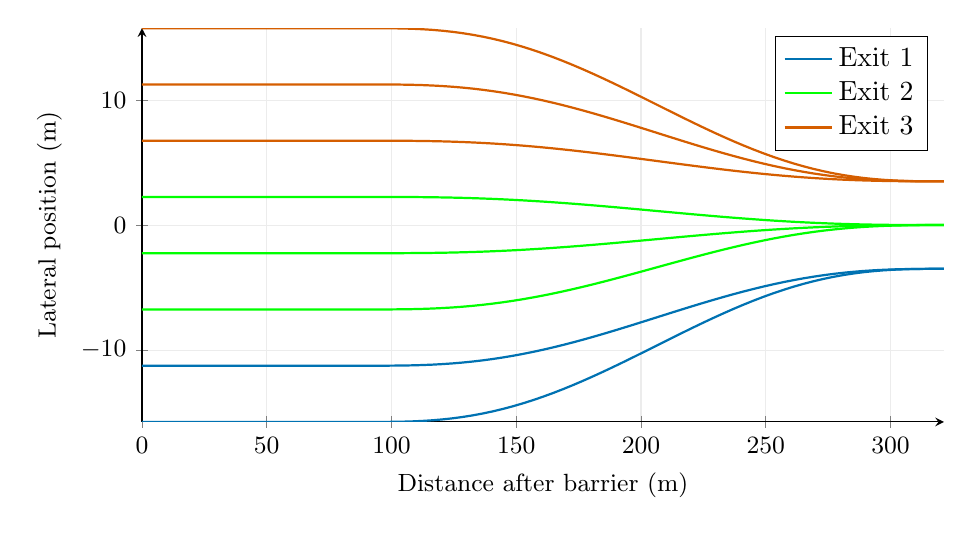
\begin{tikzpicture}\begin{axis}[width=.84\linewidth,height=5.0cm,scale only axis,xlabel={Distance after barrier (m)},ylabel={Lateral position (m)},axis lines=left,grid=major,grid style={gray!15},tick label style={font=\small},label style={font=\small}]\addplot[thick,main,no marks] coordinates {(0.0000,-15.75000) (4.0180,-15.75000) (8.0360,-15.75000) (12.0540,-15.75000) (16.0720,-15.75000) (20.0900,-15.75000) (24.1080,-15.75000) (28.1260,-15.75000) (32.1440,-15.75000) (36.1620,-15.75000) (40.1800,-15.75000) (44.1980,-15.75000) (48.2160,-15.75000) (52.2340,-15.75000) (56.2520,-15.75000) (60.2700,-15.75000) (64.2880,-15.75000) (68.3060,-15.75000) (72.3240,-15.75000) (76.3420,-15.75000) (80.3600,-15.75000) (84.3780,-15.75000) (88.3960,-15.75000) (92.4140,-15.74999) (96.4320,-15.74879) (100.4500,-15.74306) (104.4680,-15.72959) (108.4860,-15.70551) (112.5040,-15.66836) (116.5220,-15.61598) (120.5400,-15.54660) (124.5580,-15.45872) (128.5760,-15.35119) (132.5940,-15.22311) (136.6120,-15.07389) (140.6300,-14.90320) (144.6480,-14.71094) (148.6660,-14.49728) (152.6840,-14.26256) (156.7020,-14.00738) (160.7200,-13.73249) (164.7380,-13.43885) (168.7560,-13.12756) (172.7740,-12.79988) (176.7920,-12.45720) (180.8100,-12.10103) (184.8280,-11.73299) (188.8460,-11.35479) (192.8640,-10.96821) (196.8820,-10.57511) (200.9000,-10.17739) (204.9180,-9.77698) (208.9360,-9.37582) (212.9540,-8.97588) (216.9720,-8.57910) (220.9900,-8.18741) (225.0080,-7.80270) (229.0260,-7.42680) (233.0440,-7.06148) (237.0620,-6.70844) (241.0800,-6.36926) (245.0980,-6.04542) (249.1160,-5.73830) (253.1340,-5.44911) (257.1520,-5.17892) (261.1700,-4.92864) (265.1880,-4.69898) (269.2060,-4.49048) (273.2240,-4.30344) (277.2420,-4.13797) (281.2600,-3.99392) (285.2780,-3.87089) (289.2960,-3.76821) (293.3140,-3.68493) (297.3320,-3.61982) (301.3500,-3.57132) (305.3680,-3.53754) (309.3860,-3.51628) (313.4040,-3.50495) (317.4220,-3.50064) (321.4400,-3.50000)};\addlegendentry{Exit 1}\addplot[thick,main,no marks,forget plot] coordinates {(0.0000,-11.25000) (4.0180,-11.25000) (8.0360,-11.25000) (12.0540,-11.25000) (16.0720,-11.25000) (20.0900,-11.25000) (24.1080,-11.25000) (28.1260,-11.25000) (32.1440,-11.25000) (36.1620,-11.25000) (40.1800,-11.25000) (44.1980,-11.25000) (48.2160,-11.25000) (52.2340,-11.25000) (56.2520,-11.25000) (60.2700,-11.25000) (64.2880,-11.25000) (68.3060,-11.25000) (72.3240,-11.25000) (76.3420,-11.25000) (80.3600,-11.25000) (84.3780,-11.25000) (88.3960,-11.25000) (92.4140,-11.24999) (96.4320,-11.24923) (100.4500,-11.24561) (104.4680,-11.23708) (108.4860,-11.22185) (112.5040,-11.19835) (116.5220,-11.16521) (120.5400,-11.12132) (124.5580,-11.06572) (128.5760,-10.99769) (132.5940,-10.91666) (136.6120,-10.82226) (140.6300,-10.71427) (144.6480,-10.59264) (148.6660,-10.45746) (152.6840,-10.30897) (156.7020,-10.14753) (160.7200,-9.97362) (164.7380,-9.78785) (168.7560,-9.59091) (172.7740,-9.38360) (176.7920,-9.16680) (180.8100,-8.94146) (184.8280,-8.70862) (188.8460,-8.46935) (192.8640,-8.22479) (196.8820,-7.97609) (200.9000,-7.72447) (204.9180,-7.47115) (208.9360,-7.21735) (212.9540,-6.96433) (216.9720,-6.71331) (220.9900,-6.46550) (225.0080,-6.22211) (229.0260,-5.98430) (233.0440,-5.75318) (237.0620,-5.52983) (241.0800,-5.31524) (245.0980,-5.11037) (249.1160,-4.91607) (253.1340,-4.73311) (257.1520,-4.56217) (261.1700,-4.40383) (265.1880,-4.25854) (269.2060,-4.12663) (273.2240,-4.00830) (277.2420,-3.90362) (281.2600,-3.81248) (285.2780,-3.73464) (289.2960,-3.66968) (293.3140,-3.61700) (297.3320,-3.57580) (301.3500,-3.54512) (305.3680,-3.52375) (309.3860,-3.51030) (313.4040,-3.50313) (317.4220,-3.50040) (321.4400,-3.50000)};\addplot[thick,green,no marks] coordinates {(0.0000,-6.75000) (4.0180,-6.75000) (8.0360,-6.75000) (12.0540,-6.75000) (16.0720,-6.75000) (20.0900,-6.75000) (24.1080,-6.75000) (28.1260,-6.75000) (32.1440,-6.75000) (36.1620,-6.75000) (40.1800,-6.75000) (44.1980,-6.75000) (48.2160,-6.75000) (52.2340,-6.75000) (56.2520,-6.75000) (60.2700,-6.75000) (64.2880,-6.75000) (68.3060,-6.75000) (72.3240,-6.75000) (76.3420,-6.75000) (80.3600,-6.75000) (84.3780,-6.75000) (88.3960,-6.75000) (92.4140,-6.74999) (96.4320,-6.74933) (100.4500,-6.74618) (104.4680,-6.73875) (108.4860,-6.72549) (112.5040,-6.70501) (116.5220,-6.67615) (120.5400,-6.63792) (124.5580,-6.58950) (128.5760,-6.53025) (132.5940,-6.45967) (136.6120,-6.37745) (140.6300,-6.28340) (144.6480,-6.17746) (148.6660,-6.05972) (152.6840,-5.93039) (156.7020,-5.78978) (160.7200,-5.63831) (164.7380,-5.47651) (168.7560,-5.30498) (172.7740,-5.12442) (176.7920,-4.93560) (180.8100,-4.73934) (184.8280,-4.53654) (188.8460,-4.32815) (192.8640,-4.11514) (196.8820,-3.89853) (200.9000,-3.67938) (204.9180,-3.45874) (208.9360,-3.23770) (212.9540,-3.01732) (216.9720,-2.79869) (220.9900,-2.58286) (225.0080,-2.37087) (229.0260,-2.16375) (233.0440,-1.96245) (237.0620,-1.76791) (241.0800,-1.58102) (245.0980,-1.40258) (249.1160,-1.23335) (253.1340,-1.07400) (257.1520,-0.92512) (261.1700,-0.78721) (265.1880,-0.66066) (269.2060,-0.54577) (273.2240,-0.44271) (277.2420,-0.35154) (281.2600,-0.27216) (285.2780,-0.20437) (289.2960,-0.14779) (293.3140,-0.10190) (297.3320,-0.06602) (301.3500,-0.03930) (305.3680,-0.02069) (309.3860,-0.00897) (313.4040,-0.00273) (317.4220,-0.00035) (321.4400,0.00000)};\addlegendentry{Exit 2}\addplot[thick,green,no marks,forget plot] coordinates {(0.0000,-2.25000) (4.0180,-2.25000) (8.0360,-2.25000) (12.0540,-2.25000) (16.0720,-2.25000) (20.0900,-2.25000) (24.1080,-2.25000) (28.1260,-2.25000) (32.1440,-2.25000) (36.1620,-2.25000) (40.1800,-2.25000) (44.1980,-2.25000) (48.2160,-2.25000) (52.2340,-2.25000) (56.2520,-2.25000) (60.2700,-2.25000) (64.2880,-2.25000) (68.3060,-2.25000) (72.3240,-2.25000) (76.3420,-2.25000) (80.3600,-2.25000) (84.3780,-2.25000) (88.3960,-2.25000) (92.4140,-2.25000) (96.4320,-2.24978) (100.4500,-2.24873) (104.4680,-2.24625) (108.4860,-2.24183) (112.5040,-2.23500) (116.5220,-2.22538) (120.5400,-2.21264) (124.5580,-2.19650) (128.5760,-2.17675) (132.5940,-2.15322) (136.6120,-2.12582) (140.6300,-2.09447) (144.6480,-2.05915) (148.6660,-2.01991) (152.6840,-1.97680) (156.7020,-1.92993) (160.7200,-1.87944) (164.7380,-1.82550) (168.7560,-1.76833) (172.7740,-1.70814) (176.7920,-1.64520) (180.8100,-1.57978) (184.8280,-1.51218) (188.8460,-1.44272) (192.8640,-1.37171) (196.8820,-1.29951) (200.9000,-1.22646) (204.9180,-1.15291) (208.9360,-1.07923) (212.9540,-1.00577) (216.9720,-0.93290) (220.9900,-0.86095) (225.0080,-0.79029) (229.0260,-0.72125) (233.0440,-0.65415) (237.0620,-0.58930) (241.0800,-0.52701) (245.0980,-0.46753) (249.1160,-0.41112) (253.1340,-0.35800) (257.1520,-0.30837) (261.1700,-0.26240) (265.1880,-0.22022) (269.2060,-0.18192) (273.2240,-0.14757) (277.2420,-0.11718) (281.2600,-0.09072) (285.2780,-0.06812) (289.2960,-0.04926) (293.3140,-0.03397) (297.3320,-0.02201) (301.3500,-0.01310) (305.3680,-0.00690) (309.3860,-0.00299) (313.4040,-0.00091) (317.4220,-0.00012) (321.4400,0.00000)};\addplot[thick,green,no marks,forget plot] coordinates {(0.0000,2.25000) (4.0180,2.25000) (8.0360,2.25000) (12.0540,2.25000) (16.0720,2.25000) (20.0900,2.25000) (24.1080,2.25000) (28.1260,2.25000) (32.1440,2.25000) (36.1620,2.25000) (40.1800,2.25000) (44.1980,2.25000) (48.2160,2.25000) (52.2340,2.25000) (56.2520,2.25000) (60.2700,2.25000) (64.2880,2.25000) (68.3060,2.25000) (72.3240,2.25000) (76.3420,2.25000) (80.3600,2.25000) (84.3780,2.25000) (88.3960,2.25000) (92.4140,2.25000) (96.4320,2.24978) (100.4500,2.24873) (104.4680,2.24625) (108.4860,2.24183) (112.5040,2.23500) (116.5220,2.22538) (120.5400,2.21264) (124.5580,2.19650) (128.5760,2.17675) (132.5940,2.15322) (136.6120,2.12582) (140.6300,2.09447) (144.6480,2.05915) (148.6660,2.01991) (152.6840,1.97680) (156.7020,1.92993) (160.7200,1.87944) (164.7380,1.82550) (168.7560,1.76833) (172.7740,1.70814) (176.7920,1.64520) (180.8100,1.57978) (184.8280,1.51218) (188.8460,1.44272) (192.8640,1.37171) (196.8820,1.29951) (200.9000,1.22646) (204.9180,1.15291) (208.9360,1.07923) (212.9540,1.00577) (216.9720,0.93290) (220.9900,0.86095) (225.0080,0.79029) (229.0260,0.72125) (233.0440,0.65415) (237.0620,0.58930) (241.0800,0.52701) (245.0980,0.46753) (249.1160,0.41112) (253.1340,0.35800) (257.1520,0.30837) (261.1700,0.26240) (265.1880,0.22022) (269.2060,0.18192) (273.2240,0.14757) (277.2420,0.11718) (281.2600,0.09072) (285.2780,0.06812) (289.2960,0.04926) (293.3140,0.03397) (297.3320,0.02201) (301.3500,0.01310) (305.3680,0.00690) (309.3860,0.00299) (313.4040,0.00091) (317.4220,0.00012) (321.4400,0.00000)};\addplot[thick,accent,no marks] coordinates {(0.0000,6.75000) (4.0180,6.75000) (8.0360,6.75000) (12.0540,6.75000) (16.0720,6.75000) (20.0900,6.75000) (24.1080,6.75000) (28.1260,6.75000) (32.1440,6.75000) (36.1620,6.75000) (40.1800,6.75000) (44.1980,6.75000) (48.2160,6.75000) (52.2340,6.75000) (56.2520,6.75000) (60.2700,6.75000) (64.2880,6.75000) (68.3060,6.75000) (72.3240,6.75000) (76.3420,6.75000) (80.3600,6.75000) (84.3780,6.75000) (88.3960,6.75000) (92.4140,6.75000) (96.4320,6.74968) (100.4500,6.74816) (104.4680,6.74458) (108.4860,6.73820) (112.5040,6.72834) (116.5220,6.71444) (120.5400,6.69604) (124.5580,6.67272) (128.5760,6.64419) (132.5940,6.61021) (136.6120,6.57062) (140.6300,6.52534) (144.6480,6.47433) (148.6660,6.41764) (152.6840,6.35537) (156.7020,6.28767) (160.7200,6.21474) (164.7380,6.13684) (168.7560,6.05425) (172.7740,5.96731) (176.7920,5.87640) (180.8100,5.78190) (184.8280,5.68426) (188.8460,5.58392) (192.8640,5.48136) (196.8820,5.37707) (200.9000,5.27155) (204.9180,5.16532) (208.9360,5.05889) (212.9540,4.95278) (216.9720,4.84752) (220.9900,4.74360) (225.0080,4.64153) (229.0260,4.54180) (233.0440,4.44488) (237.0620,4.35122) (241.0800,4.26123) (245.0980,4.17532) (249.1160,4.09383) (253.1340,4.01711) (257.1520,3.94543) (261.1700,3.87903) (265.1880,3.81810) (269.2060,3.76278) (273.2240,3.71316) (277.2420,3.66926) (281.2600,3.63104) (285.2780,3.59840) (289.2960,3.57116) (293.3140,3.54906) (297.3320,3.53179) (301.3500,3.51892) (305.3680,3.50996) (309.3860,3.50432) (313.4040,3.50131) (317.4220,3.50017) (321.4400,3.50000)};\addlegendentry{Exit 3}\addplot[thick,accent,no marks,forget plot] coordinates {(0.0000,11.25000) (4.0180,11.25000) (8.0360,11.25000) (12.0540,11.25000) (16.0720,11.25000) (20.0900,11.25000) (24.1080,11.25000) (28.1260,11.25000) (32.1440,11.25000) (36.1620,11.25000) (40.1800,11.25000) (44.1980,11.25000) (48.2160,11.25000) (52.2340,11.25000) (56.2520,11.25000) (60.2700,11.25000) (64.2880,11.25000) (68.3060,11.25000) (72.3240,11.25000) (76.3420,11.25000) (80.3600,11.25000) (84.3780,11.25000) (88.3960,11.25000) (92.4140,11.24999) (96.4320,11.24923) (100.4500,11.24561) (104.4680,11.23708) (108.4860,11.22185) (112.5040,11.19835) (116.5220,11.16521) (120.5400,11.12132) (124.5580,11.06572) (128.5760,10.99769) (132.5940,10.91666) (136.6120,10.82226) (140.6300,10.71427) (144.6480,10.59264) (148.6660,10.45746) (152.6840,10.30897) (156.7020,10.14753) (160.7200,9.97362) (164.7380,9.78785) (168.7560,9.59091) (172.7740,9.38360) (176.7920,9.16680) (180.8100,8.94146) (184.8280,8.70862) (188.8460,8.46935) (192.8640,8.22479) (196.8820,7.97609) (200.9000,7.72447) (204.9180,7.47115) (208.9360,7.21735) (212.9540,6.96433) (216.9720,6.71331) (220.9900,6.46550) (225.0080,6.22211) (229.0260,5.98430) (233.0440,5.75318) (237.0620,5.52983) (241.0800,5.31524) (245.0980,5.11037) (249.1160,4.91607) (253.1340,4.73311) (257.1520,4.56217) (261.1700,4.40383) (265.1880,4.25854) (269.2060,4.12663) (273.2240,4.00830) (277.2420,3.90362) (281.2600,3.81248) (285.2780,3.73464) (289.2960,3.66968) (293.3140,3.61700) (297.3320,3.57580) (301.3500,3.54512) (305.3680,3.52375) (309.3860,3.51030) (313.4040,3.50313) (317.4220,3.50040) (321.4400,3.50000)};\addplot[thick,accent,no marks,forget plot] coordinates {(0.0000,15.75000) (4.0180,15.75000) (8.0360,15.75000) (12.0540,15.75000) (16.0720,15.75000) (20.0900,15.75000) (24.1080,15.75000) (28.1260,15.75000) (32.1440,15.75000) (36.1620,15.75000) (40.1800,15.75000) (44.1980,15.75000) (48.2160,15.75000) (52.2340,15.75000) (56.2520,15.75000) (60.2700,15.75000) (64.2880,15.75000) (68.3060,15.75000) (72.3240,15.75000) (76.3420,15.75000) (80.3600,15.75000) (84.3780,15.75000) (88.3960,15.75000) (92.4140,15.74999) (96.4320,15.74879) (100.4500,15.74306) (104.4680,15.72959) (108.4860,15.70551) (112.5040,15.66836) (116.5220,15.61598) (120.5400,15.54660) (124.5580,15.45872) (128.5760,15.35119) (132.5940,15.22311) (136.6120,15.07389) (140.6300,14.90320) (144.6480,14.71094) (148.6660,14.49728) (152.6840,14.26256) (156.7020,14.00738) (160.7200,13.73249) (164.7380,13.43885) (168.7560,13.12756) (172.7740,12.79988) (176.7920,12.45720) (180.8100,12.10103) (184.8280,11.73299) (188.8460,11.35479) (192.8640,10.96821) (196.8820,10.57511) (200.9000,10.17739) (204.9180,9.77698) (208.9360,9.37582) (212.9540,8.97588) (216.9720,8.57910) (220.9900,8.18741) (225.0080,7.80270) (229.0260,7.42680) (233.0440,7.06148) (237.0620,6.70844) (241.0800,6.36926) (245.0980,6.04542) (249.1160,5.73830) (253.1340,5.44911) (257.1520,5.17892) (261.1700,4.92864) (265.1880,4.69898) (269.2060,4.49048) (273.2240,4.30344) (277.2420,4.13797) (281.2600,3.99392) (285.2780,3.87089) (289.2960,3.76821) (293.3140,3.68493) (297.3320,3.61982) (301.3500,3.57132) (305.3680,3.53754) (309.3860,3.51628) (313.4040,3.50495) (317.4220,3.50064) (321.4400,3.50000)};\end{axis}\end{tikzpicture}\caption{Order-preserving centerline paths for the selected nominal design. Curves within one group merge at its assigned exit. Release spacing is a separate control requirement.}\label{fig:paths}\end{figure}
\section{Layout selection and construction trade-offs}
We enumerate 441 layouts with payment types clustered in the order ETC, exact-change, staffed, and contiguous exit groups. The ETC-left convention follows the historical mainline guidance \cite{orientation}. An unrestricted comparison of 6,750 matrices attains the same nominal and worst-case optimum thresholds for these inputs, so clustering sacrifices no capacity optimum here. This equivalence is not asserted for other demand or geometry scenarios. Ties minimize capital cost, then the largest number of streams feeding one exit.

The cost scenario is $K_c=c_A A+\sum_t k_t N_t$, where $A=RBw_b+D(Bw_b+Lw)/2$ includes recovery and taper pavement. Equipment assumptions for staffed, exact-change and electronic booths are \$80,000, \$60,000, \$120,000. This full-build comparison excludes land acquisition, shoulders, maintenance, staffing and discounting. It cannot establish investment return or a final construction budget; land opportunity cost is added in the scenarios below.

\begin{table}[H]\centering\small\caption{Capacity and capital scenarios. Counts are staffed/exact/ETC; length includes recovery and taper. Rate columns are fluid arrival thresholds (veh/h).}\label{tab:design}\begin{tabular}{@{}llrrrr@{}}\toprule
Design & Counts & Length (m) & Cost (\$m) & Nominal & Worst\\\midrule
Initial & 3/3/2 & 321.44 & 2.388 & 3,000 & --\\
Nominal & 4/3/1 & 321.44 & 2.348 & 4,000 & 2,400.0\\
Robust & 4/2/2 & 321.44 & 2.408 & 4,000 & 2,666.7\\
Expanded & 6/3/2 & 451.44 & 3.965 & 5,100 & 4,000.0\\
\bottomrule\end{tabular}\end{table}
The nominal design increases the threshold from 3,000 to 4,000 vehicles/hour. Relative to the nominal design, the robust design retains that nominal threshold and raises the electronic-heavy threshold from 2,400 to 4,000 vehicles/hour, at an additional assumed capital cost of \$60,000. It cannot remove the cash-heavy bottleneck.

\begin{table}[H]\centering\small\caption{Contiguous exit groups of the nominal and robust designs.}\begin{tabular}{@{}lrrr@{}}\toprule
Design / group & Staffed & Exact & ETC\\\midrule
Nominal / 1 & 0 & 1 & 1\\
Nominal / 2 & 1 & 2 & 0\\
Nominal / 3 & 3 & 0 & 0\\
Robust / 1 & 0 & 0 & 1\\
Robust / 2 & 0 & 2 & 1\\
Robust / 3 & 4 & 0 & 0\\
\bottomrule\end{tabular}\end{table}
\begin{figure}[htbp]\centering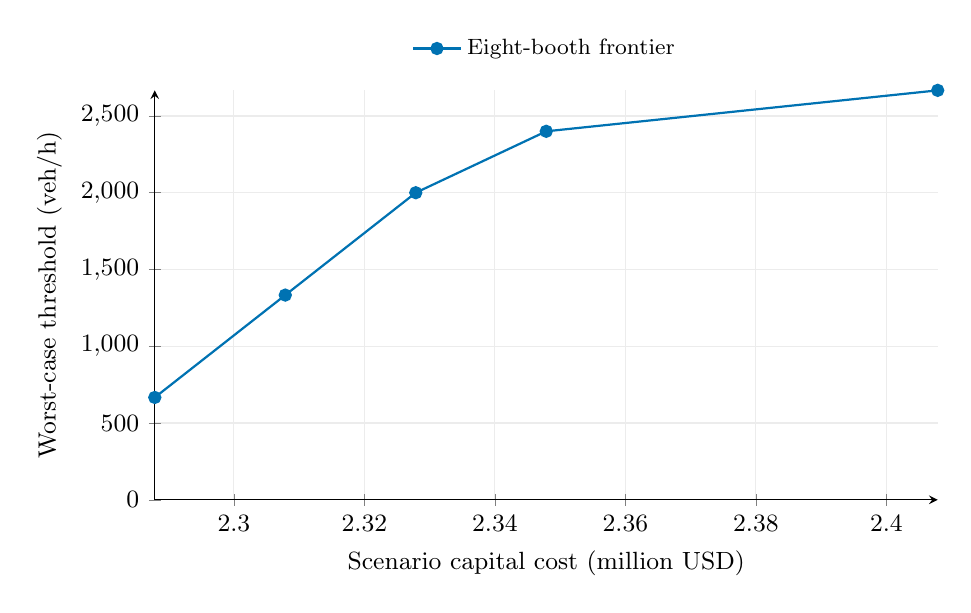
\begin{tikzpicture}\begin{axis}[width=.82\linewidth,height=5.2cm,scale only axis,axis lines=left,grid=major,grid style={gray!15},xlabel={Scenario capital cost (million USD)},ylabel={Worst-case threshold (veh/h)},ymin=0,legend style={font=\footnotesize,draw=none,at={(.5,1.05)},anchor=south,legend columns=2},tick label style={font=\small},label style={font=\small}]\addplot[thick,main,mark=*] coordinates {(2.287868,666.66667) (2.307868,1333.3333) (2.327868,2000) (2.347868,2400) (2.407868,2666.6667)};\addlegendentry{Eight-booth frontier}\end{axis}\end{tikzpicture}\caption{Nondominated cost/capacity points within the enumerated eight-booth family. Different land prices or admissible routing rules can change this frontier.}\label{fig:frontier}\end{figure}
\begin{table}[H]\centering\small\caption{Land opportunity-cost scenarios added to road and equipment costs. Column prices are USD/m$^2$: illustrative assumptions, not local quotations. Totals are in millions of USD.}\begin{tabular}{@{}lrrrr@{}}\toprule
Design & Area (m$^2$) & 0 & 200 & 1000\\\midrule
nominal & 8,639.34 & 2.348 & 4.076 & 10.987\\
robust & 8,639.34 & 2.408 & 4.136 & 11.047\\
expanded & 15,326.28 & 3.965 & 7.031 & 19.292\\
\bottomrule\end{tabular}\end{table}
Expansion needs 6,686.94 m$^2$ more modeled pavement footprint than the robust eight-booth option. Each additional dollar per square meter of land opportunity cost therefore adds \$6,686.94 to the expansion premium. Equal-area eight-booth designs retain their equipment-cost difference, while higher land cost makes expansion more expensive. Without project life, traffic revenue or a delay valuation, these scenarios cannot establish an investment break-even point. The footprint still excludes shoulders and approach-side land.

\section{An infeasibility result and a feasible expansion}
For a target demand $q$, a necessary condition under every payment mixture is $N_t\mu_t\ge q\max_s p_{st}$. Therefore $N_t\ge\lceil q\max_s p_{st}/\mu_t\rceil$. This gives a lower bound independent of lane routing and geometric preferences.

At 3,600 vehicles/hour, the three type minima are 6, 3, 2 booths, totaling 11. Hence no eight-, nine- or ten-booth arrangement with the same service capabilities can accommodate all three mixtures. This is stronger than failing to find a good layout: the payment requirements alone exclude those totals.

A layout with those 11 booths and 3 exits is feasible. Its scenario thresholds are nominal: 5,100.0 vehicles/hour, cash heavy: 4,000.0 vehicles/hour, electronic heavy: 4,000.0 vehicles/hour. Its departure zone, including recovery and taper, is 451.44 m long, with assumed full-build cost \$3,965,256. We search only allocations of the necessary booth-count vector for this expansion; the capacity certificate proves feasibility, while the smallest count follows from the lower bound. We do not claim minimum cost over all larger facilities or all road geometries.

The robust eight-booth threshold is 2,666.7 vehicles/hour. A rate strictly above it would require at least five staffed, two exact-change and two electronic booths under the declared scenario maxima, exceeding eight in total. The selected design reaches the bound in the fluid model. The nominal threshold is likewise conditional on the three service means and nominal shares, rather than a universal property of eight booths.

\section{Light and heavy traffic: finite-episode queues}
Arrivals form a Poisson stream for 30 minutes and are then stopped while the queues drain. Payment types are independent marks with the specified scenario probabilities. Lognormal service times preserve the assumed means and coefficients of variation. For each scenario/load combination we use the same arrivals, payment marks, service draws and routing uniforms across all designs. The eight preselected seeds are 641, 642, 643, 644, 645, 646, 647, 648. These replications quantify variation in the model, not uncertainty about real traffic.

The LP routing witness gives each compatible booth a fixed fraction of its type demand. A booth is a single server. After service and recovery, a vehicle travels the taper and joins its receiving lane; discharge times satisfy $d_k=\max(a_k,d_{k-1}+h)$, where $a_k=r_k+T$ is the free-arrival time at the taper end. Total waiting excludes the vehicle's realized service and free recovery/traversal time. All arrivals are retained through clearance, so vehicles remaining at the demand horizon are not dropped. This section first assumes unlimited holding; the next tests blocking.

\begin{table}[H]\centering\small\caption{Eight-replication means with unlimited holding. Waiting includes arrivals through drainage; output and clearance refer to heavy demand. Output counts only demand-window departures. Wait and clearance are in seconds; output is in veh/h.}\label{tab:queues}\begin{tabular}{@{}llrrrr@{}}\toprule
Payment mix & Design & Light wait & Heavy wait & Output & Clearance\\\midrule
nominal & baseline & 2.1 & 66.1 & 3,306 & 568.1\\
 & nominal & 1.6 & 21.8 & 3,442 & 164.3\\
 & robust & 1.6 & 21.8 & 3,442 & 164.3\\
 & expanded & 1.2 & 8.3 & 3,452 & 90.2\\
cash heavy & baseline & 5.5 & 314.9 & 2,808 & 1,616.9\\
 & nominal & 3.3 & 170.5 & 3,006 & 849.5\\
 & robust & 3.3 & 170.4 & 3,006 & 849.5\\
 & expanded & 2.1 & 21.7 & 3,405 & 175.8\\
electronic heavy & baseline & 1.0 & 337.8 & 2,620 & 930.9\\
 & nominal & 1.5 & 358.5 & 2,568 & 935.5\\
 & robust & 0.6 & 7.8 & 3,483 & 52.9\\
 & expanded & 0.6 & 7.6 & 3,458 & 65.6\\
\bottomrule\end{tabular}\end{table}
Under nominal heavy demand, mean waiting decreases from 66.1 s to 21.8 s. Under cash-heavy demand, even the robust eight-booth option has mean waiting 170.4 s because demand exceeds its threshold; finite simulation cannot convert overload into stability. The expanded layout reduces that mean to 21.7 s, but the remaining wait warns against operating close to capacity.

The paired nominal-heavy mean reduction is 44.3 s, with an approximate 95\% Student-$t$ interval [29.0, 59.5] s over the eight replications. This interval describes Monte Carlo variation under the model, not uncertainty in service means, driver compliance or road behavior. Light-traffic differences are much smaller, so this improvement is not a uniform reduction for every operating condition.

\section{When additional booths make blocking worse}
Let $K$ be the number of downstream occupancy slots in each exit group, counting vehicles from toll release until exit, including travel and waiting. If the group is full, a vehicle that has completed service remains at its booth, preventing the next service. Once a vehicle exits, the earliest blocked completion is admitted. Thus finite occupancy can reduce toll service itself. The slots are an abstract resource, not a calibrated geometric vehicle count; the event model still does not resolve lane-changing collisions.

For free traversal times $\tau_t$, a stationary rate requires $\sum_t x_{gt}\tau_t/3600\le K$ for every group, because waiting can only increase occupancy. Minimizing $K$ over \eqref{eq:flow} gives a necessary holding bound. It excludes waiting and stochastic bursts, so satisfying it is not sufficient. Conversely, a design below this bound cannot sustain the target rate under the modeled travel times, regardless of routing.

\begin{table}[H]\centering\small\caption{Necessary per-group occupancy at the heavy demand. Infeasible service demand means no amount of holding fixes the payment constraint.}\begin{tabular}{@{}llrr@{}}\toprule
Design & Payment mix & Continuous lower bound & Integer minimum\\\midrule
robust & nominal & 12.0004 & 13\\
robust & cash heavy & infeasible service demand & --\\
robust & electronic heavy & 14.8398 & 15\\
expanded & nominal & 16.5504 & 17\\
expanded & cash heavy & 20.0576 & 21\\
expanded & electronic heavy & 20.6898 & 21\\
\bottomrule\end{tabular}\end{table}
\begin{table}[H]\centering\small\caption{Finite-occupancy heavy-demand experiments, eight paired seeds. The eight-booth column uses the robust design. Waiting covers drainage; output covers the demand window.}\begin{tabular}{@{}rlrrr@{}}\toprule
$K$ & Payment mix & 8-booth wait (s) & 11-booth wait (s) & 11-booth output\\\midrule
4 & nominal & 1,740.7 & 2,688.3 & 880\\
4 & cash heavy & 2,070.9 & 3,091.9 & 872\\
4 & electronic heavy & 2,217.8 & 3,421.1 & 877\\
16 & nominal & 21.9 & 54.3 & 3,302\\
16 & cash heavy & 172.4 & 191.3 & 2,896\\
16 & electronic heavy & 14.8 & 243.9 & 2,750\\
64 & nominal & 21.8 & 8.3 & 3,452\\
64 & cash heavy & 170.4 & 21.7 & 3,405\\
64 & electronic heavy & 7.8 & 7.6 & 3,458\\
\bottomrule\end{tabular}\end{table}
At $K=16$, nominal heavy-traffic waiting is 21.9 s for the robust eight-booth design but 54.3 s for the expansion. At $K=64$, the expansion wait falls to 8.3 s. More booths require a wider and longer taper; vehicles occupy the downstream corridor longer, so expansion without matching holding resources can worsen delay. This is a conditional queueing mechanism, not an empirical prediction for a particular plaza.

\begin{figure}[htbp]\centering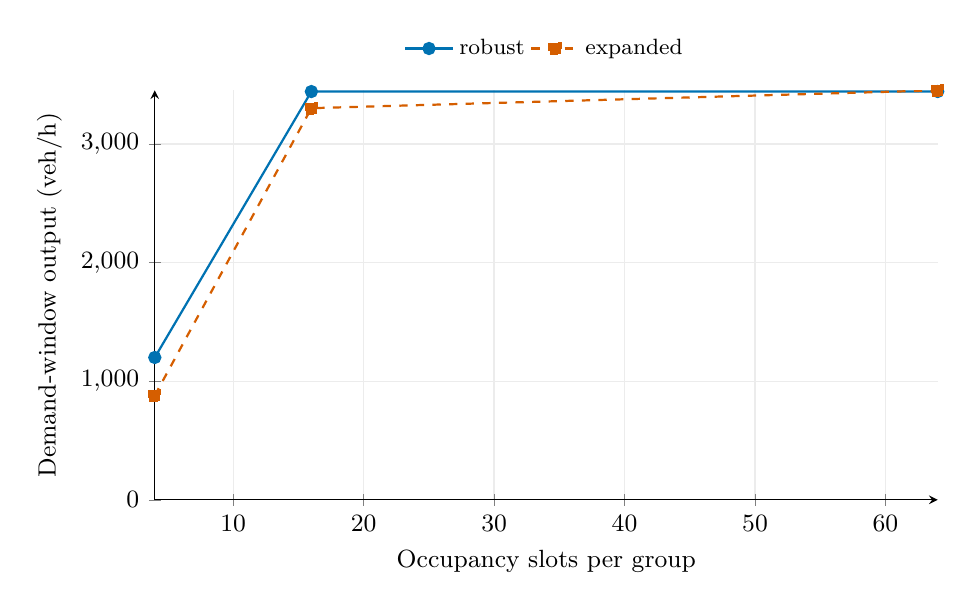
\begin{tikzpicture}\begin{axis}[width=.82\linewidth,height=5.2cm,scale only axis,axis lines=left,grid=major,grid style={gray!15},xlabel={Occupancy slots per group},ylabel={Demand-window output (veh/h)},ymin=0,legend style={font=\footnotesize,draw=none,at={(.5,1.05)},anchor=south,legend columns=2},tick label style={font=\small},label style={font=\small}]\addplot[thick,main,mark=*] coordinates {(4,1200) (16,3442.25) (64,3442.5)};\addlegendentry{robust}\addplot[thick,accent,dashed,mark=square*] coordinates {(4,879.75) (16,3302) (64,3452.25)};\addlegendentry{expanded}\end{axis}\end{tikzpicture}\caption{Nominal heavy-demand output with finite occupancy. These are transient observed rates, distinct from the compatible-flow arrival thresholds.}\label{fig:buffers}\end{figure}
We also tested an actual-demand minimax resource-load routing objective. It slightly improves some conditions but worsens nominal-design waiting in the cash-heavy overload case. A smaller maximum utilization is therefore not equivalent to smaller mean waiting. We retain the capacity-witness routing for this comparison and archive the rejected candidate; no claim of minimum-delay routing is made.

\section{Automated vehicles and sensitivity of the recommendation}
Let $a$ be the autonomous-vehicle fraction. If neighboring vehicle types are independently mixed and only an AV--AV pair uses the shorter headway, the scenario mean is $h(a)=h_H(1-a^2)+h_Aa^2$. No toll-service advantage is granted merely because a vehicle is autonomous. This isolates whether the bottleneck is at the payment barrier or the receiving lanes; real platooning or different mixed-pair behavior would require another headway model.

\begin{table}[H]\centering\small\caption{Nominal-payment thresholds as AV share changes. All booths and toll-service assumptions stay fixed.}\begin{tabular}{@{}lrrrrr@{}}\toprule
AV share & Headway (s) & Initial & Nominal & Robust & Expanded\\\midrule
0\% & 2.000 & 3,000 & 4,000 & 4,000 & 5,100\\
25\% & 1.931 & 3,000 & 4,000 & 4,000 & 5,164\\
50\% & 1.725 & 3,000 & 4,000 & 4,000 & 5,387\\
75\% & 1.381 & 3,000 & 4,000 & 4,000 & 5,906\\
100\% & 0.900 & 3,000 & 4,000 & 4,000 & 6,000\\
\bottomrule\end{tabular}\end{table}
\begin{figure}[htbp]\centering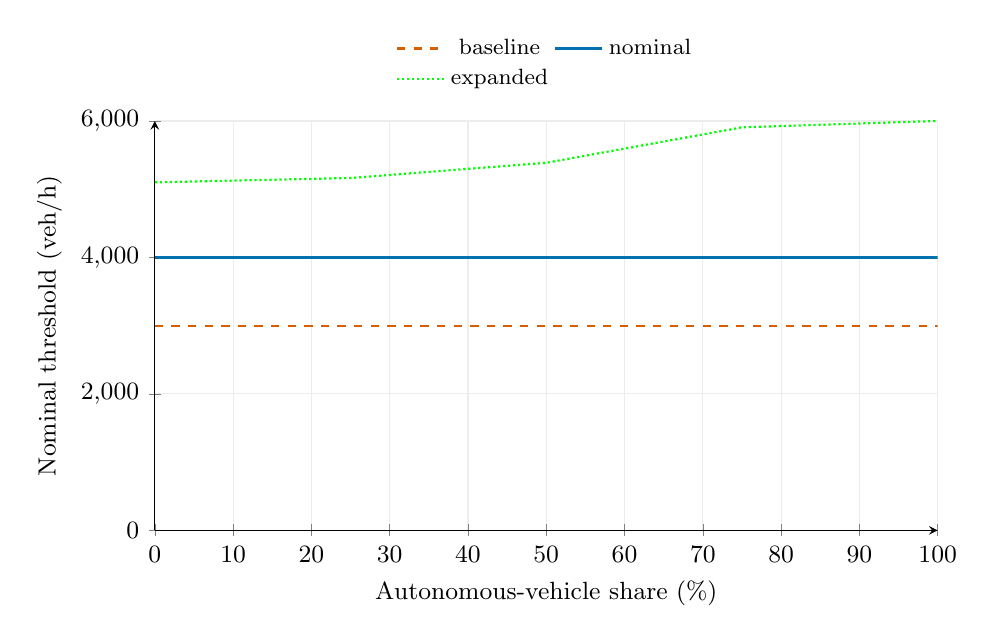
\begin{tikzpicture}\begin{axis}[width=.82\linewidth,height=5.2cm,scale only axis,axis lines=left,grid=major,grid style={gray!15},xlabel={Autonomous-vehicle share (\%)},ylabel={Nominal threshold (veh/h)},ymin=0,legend style={font=\footnotesize,draw=none,at={(.5,1.05)},anchor=south,legend columns=2},tick label style={font=\small},label style={font=\small}]\addplot[thick,accent,dashed] coordinates {(0,3000) (25,3000) (50,3000) (75,3000) (100,3000)};\addlegendentry{baseline}\addplot[thick,main,solid] coordinates {(0,4000) (25,4000) (50,4000) (75,4000) (100,4000)};\addlegendentry{nominal}\addplot[thick,green,densely dotted] coordinates {(0,5100) (25,5164.0777) (50,5386.9565) (75,5906.3348) (100,6000)};\addlegendentry{expanded}\end{axis}\end{tikzpicture}\caption{Headway improvement matters only when an exit-related cut is limiting. A flat curve means that the service/compatibility bottleneck remains.}\label{fig:av}\end{figure}
The initial layout and nominal eight-booth design are payment-limited across these nominal AV scenarios. An autonomous fleet can therefore increase receiving-lane capability without improving their total threshold. This does not mean automation has no safety or operational value; those outcomes are outside the capacity calculation. It means automation alone is not the remedy for this specified service bottleneck.

Equation~\eqref{eq:cut} also supplies exact payment-share thresholds. Holding all else fixed, a set $S$ overloads once $p(S)>\sum_g\min(C_g,\sum_{t\in S}n_{gt}\mu_t)/q$. Such inequalities are actionable: before adding pavement, measure the relevant payment proportions and test which cut is active. The scenario frontier should be recomputed when mean service or allowed routing changes. The sensitivity calculation uses the mean headway as a deterministic exit interval; it does not simulate AV pair sequences or platoon correlations. A monetary preference between robustness and lower cost remains a decision for the authority, not a number inferred from a synthetic objective.

\begin{table}[H]\centering\small\caption{Slower-service stress test: conditional thresholds (veh/h). The layouts are held fixed, not reoptimized.}\begin{tabular}{@{}lrrr@{}}\toprule
Design & Nominal mix & Cash-heavy & Electronic-heavy\\\midrule
baseline & 2,400.0 & 1,600.0 & 2,400.0\\
nominal & 3,000.0 & 2,133.3 & 1,600.0\\
robust & 2,400.0 & 2,057.1 & 3,200.0\\
expanded & 3,600.0 & 3,085.7 & 3,200.0\\
\bottomrule\end{tabular}\end{table}
With assumed service means of 15/10/3 seconds, the expanded layout no longer meets heavy demand in every mixture. The payment-only lower count becomes 7/4/3 booths, totaling 14. This stress calculation establishes a necessary count only; no layout at that count has been constructed or checked. The eleven-booth recommendation is conditional on the original service scenario.

\section{Verification, strengths and remaining limits}
An independent network-flow implementation checks every reported selected-layout threshold at the threshold and one vehicle/hour above it. The routing witnesses are checked for payment conservation, booth bounds and exit bounds. A separate exhaustive search over type totals verifies the minimum robust booth count. Analytic derivative maxima establish the path bounds, with dense numerical samples checking the generated geometry and its ordering. The queue experiment checks vehicle conservation and retains residual queues through clearance.

A separate reviewer implementation compared 256 randomized cut calculations with an independently formulated LP, checked queue examples by hand, and reproduced unlimited holding with nonbinding finite occupancy. An analytic payment-subset occupancy bound and explicit feasible routing independently attain each expanded-layout slot lower bound. These are author-external agent checks within the same model family, not human or field verification. Entry and exit metering equivalence was checked against finite-event traces without changing the numerical trajectories.

These checks have different scopes. A maximum-flow calculation verifies the conditional network result; it cannot show that drivers obey route guidance. A geometrically ordered set of centerlines does not constitute a crash model. Replication consistency cannot supply calibration data. FHWA describes calibration against capacity and performance observations; our report has no such observations and therefore does not describe the model as field-validated \cite{fhwa}.

The main strength is an interpretable bottleneck certificate linking payment mix to lane design. It both constructs feasible improvements and proves when a requested demand cannot be served with the given booth count. The main weakness is the absence of site calibration and a spatial interaction model. Finite occupancy and simple acceleration are now included, but the occupancy slots have not been mapped to safe physical storage. Open-loop routing, heavy vehicles, driver compliance and land constraints can change a practical preference even when the flow inequalities remain correct.

\section{Recommendation}
For the nominal payment mixture, choose the 4,000-vehicle/hour layout when capital is the main secondary criterion. If payment proportions may shift toward electronic collection, the robust eight-booth alternative buys broader service compatibility for an assumed \$60,000 increase. Neither option is a reliable way to serve 3,600 vehicles/hour under the cash-heavy mixture. For that service requirement across all three mixtures, the model requires at least 11 booths and supplies one feasible allocation.

Expansion is conditional on matching downstream space: in nominal heavy traffic, the eleven-booth design waits 54.3 s at 16 slots per group, compared with 21.9 s for the robust eight-booth design. Slower service also defeats the eleven-booth guarantee. Neither booth count nor a necessary occupancy bound alone is a construction specification.

Use channelized, order-preserving fan-in paths and a receiving-lane discharge rule, but validate holding space and vehicle interactions before fixing the construction drawing. Collect observed payment shares, service distributions and queue discharge rates before selecting the final booth mix. The most valuable operational change is the one that relaxes the active bottleneck; extra exit capacity is ineffective while the payment cut remains binding.

\clearpage\section*{Letter to the New Jersey Turnpike Authority}
\addcontentsline{toc}{section}{Letter to the New Jersey Turnpike Authority}
\noindent Dear Members of the Authority,

We recommend treating a toll plaza as a set of payment-compatible services connected to receiving traffic lanes. The number of open booths by itself can be misleading: unused electronic capacity cannot process a driver who requires a staffed booth. The operating plan should identify the limiting payment or exit group before adding pavement or changing discharge speeds.

For the illustrative eight-booth, three-lane facility, our nominal arrangement raises the modeled capacity threshold from 3,000 to 4,000 vehicles per hour. It uses 4/3/1 staffed/exact-change/electronic booths, allocated among contiguous exit groups. Each group receives compatible demand and is metered at the taper entrance. A parallel recovery section of 91.44 meters precedes a smooth taper of 230 meters, which meets our assumed slope and lateral-acceleration limits at 10 meters per second.

The nominal design is not the best choice for every payment mixture. An eight-booth robust alternative costs an additional assumed \$60,000 and handles an electronic-heavy mixture better. Under cash-heavy demand, however, every eight-booth design remains limited. Serving 3,600 vehicles per hour under all three studied mixtures requires at least 11 booths with the stated service capabilities. We provide a feasible expanded arrangement rather than suggesting that shorter headways alone can solve this constraint.

In the nominal heavy-traffic experiments, mean waiting falls from 66.1 to 21.8 seconds. These figures come from specified synthetic demand episodes, not observations of your road. They identify a promising change to test; they are not forecasts of achieved delay or accident reduction.

Expansion also lengthens traversal. At 16 downstream slots per group, its nominal heavy-traffic waiting rises to 54.3 seconds, above the robust eight-booth alternative. At 64 slots per group, the expanded design's nominal heavy-traffic mean waiting falls to 8.3 seconds, removing this particular modeled penalty in the tested scenario. We therefore recommend testing a combined booth-and-storage plan rather than approving extra booths in isolation.

Before construction, price the required land, measure payment proportions and service times, test whether drivers follow route guidance, and check finite holding space and vehicle trajectories. Our idealized centerlines and release intervals address specific kinematic concerns, but do not estimate crashes or replace engineering standards. A pilot can first change signs and booth assignments; major pavement expansion should follow only when the observed limiting mechanism justifies it.

\noindent Respectfully,\\Team 7391857
\clearpage
\begin{thebibliography}{9}
\bibitem{comap} COMAP. 2017 MCM Problem B: Merge After Toll. 2017. Official problem statement.
\url{https://www.contest.comap.com/undergraduate/contests/mcm/contests/2017/problems/2017_MCM_Problem_B.pdf}.
\bibitem{fhwa} Federal Highway Administration. Traffic Analysis Toolbox, Volume III: Guidelines for Applying Traffic Microsimulation Modeling Software. 2004, Chapter 5, Model Calibration. FHWA-HRT-04-040.
\url{https://ops.fhwa.dot.gov/trafficanalysistools/tat_vol3/sect5.htm}.
\bibitem{departure} Wilbur Smith Associates, for the Federal Highway Administration. State of the Practice and Recommendations on Traffic Control Strategies at Toll Plazas. June 2006, Section 6.4.2, Departure Zones.
\url{https://mutcd.fhwa.dot.gov/rpt/tcstoll/chapter642.htm}.
\bibitem{orientation} Wilbur Smith Associates, for the Federal Highway Administration. State of the Practice and Recommendations on Traffic Control Strategies at Toll Plazas. June 2006, Section 2.2.4, Toll Lane Configuration.
\url{https://mutcd.fhwa.dot.gov/rpt/tcstoll/chapter224.htm}.
\end{thebibliography}
\clearpage\section*{Report on Use of AI Tools}
\addcontentsline{toc}{section}{Report on Use of AI Tools}
An OpenAI Codex agent conducted the problem interpretation, mathematical modeling, programming, numerical experiments and English writing in one delegated research episode. The agent selected the historical task and read its official statement and general FHWA guidance. No same-problem submitted solution or judges' commentary was consulted during this episode. Possible exposure during model pretraining is unknown.

The user supplied the plugin-development objective and authorized local research; the user did not supply this case's model choices or perform its mathematical verification. Other agent roles of the same model family reviewed the numerical tools and, where recorded in the accompanying archive, the case. Such review is not human verification or independent field validation.

Python and its scientific libraries performed layout enumeration, flow construction and queue calculations. LaTeX produced this document. Numerical verification checks the model against distinct algorithms and analytic conditions; it does not establish empirical safety or traffic calibration. The accompanying research archive retains the available run receipts, failed candidates and review scope. Full raw model input/output transcripts are not available in that archive, and no complete interaction log is reconstructed from summaries.
\end{document}

